\section{Piecewise Aggregate Approximation (PAA)}
Following proposed time-series similarity methods based on Fourier, SVD and Haar wavelet transforms Faloutsos et al \cite{citeulike:4344279}, Yi \& Faloutsos \cite{citeulike:2946589} and Keogh et al \cite{citeulike:3000416} followed with Piecewise Aggregate Approximation (PAA) (aka Piecewise Linear (PLA) or Piecewise Constant (PCA)) based approaches for the time-series dimensionality reduction. It was shown that surprisingly simple PAA-based methods outperforms any other sophisticated technique up to date.

As mentioned, the PAA method is surprisingly simple as opposite to others and it approximates the time-series $X$ of length $n$ into vector $\bar{X} = ( \bar{x}_{1}, ..., \bar{x}_{M} )$ of length $M$ where each of $\bar{x_{i}}$ is calculated by following the next formula:
\begin{equation}
\bar{x}_{i} = \frac{M}{n} \sum_{j=n/M(i-1)+1}^{(n/M)i} x_{j}
\label{eq:paa}
\end{equation}
Which simply means that in order to reduce the dimensionality from $n$ to $M$ at first we divide the original time-series in the $M$ equi-sized frames and secondly compute the mean values for each frame. The sequence assembled from the mean values is the PAA transform of the original time-series. It was shown by Keogh et al that the complexity of the PAA transform can be reduced from $O(NM)$ (\ref{eq:paa}) to $O(Mm)$ where $m$ is the number of the sliding windows. The satisfaction of the transform to bounding condition in order to guarantee no false dismissals was
also shown by Yi \& Faloutsos and Keogh et al by introducing the distance:
\begin{equation}
D_{PAA}(\bar{X}, \bar{Y}) \equiv \sqrt{\frac{n}{M}} \sqrt{ \sum_{i=1}^{M} 
\left(  \bar{x}_{i} - \bar{y}_{i} \right)}
\label{eq:paa_distnace}
\end{equation}
and showing that $D_{PAA}(\bar{X}, \bar{Y}) \leq D(X,Y)$.

Concluding the PAA review we should note that PAA is very similar to Haar-wavelet based approach \cite{citeulike:4384535} as shown at the Figure \ref{fig:paa_comparison}. Another nice feature of PAA based approach for indexing and querying time-series databases with longer or shorter query sequences was shown by Keogh et al in \cite{citeulike:3000416}.
\begin{figure}[tbp]
   \centering
   \includegraphics[height=95mm]{paa_comparison.eps}
   %%{seriesheatmap}
   \caption{The combination of figures from \cite{citeulike:3000416} depicts different approaches for the time-series approximation (decomposition): a) the time-series spectral approximation (Fourier); b) SVD-based approximation; c) Haar-wavelet based approximation; d) Piecewise Aggregate Approximation where transformed values shown as ``box'' basis functions.}
   \label{fig:paa_comparison}
\end{figure} 

Overall the PAA-transform based approach to the time-series similarity problem was found very competitive in the precision to the Fourier-based, SVD and wavelets while outperformin all cometitors in the speed of index building, constant time of insertions and deletion from index (in case of SVD for example we have to rebuild the whole matrix) and ability to handle queries of the unequal to index dimensionality size. Also Keogh et al has shown the PAA ability to handle the weighted Euclidean distance metrics allowing implementation of more sophisticated querying techniques like relevance feedback \cite{citeulike:4406444}.
